
{\actuality}При облучении газа атомов щелочных металлов встречными бихроматическими лазерными пучками, в профиле поглощения образуется высококонтрастный субдоплеровский резонанс.
Первое сообщение о наблюдении данного эффекта было представлено в работе \autocite{hafiz2016}.
В этой работе авторы использовали линейно поляризованные пучки моно-- и би-- хроматического лазерного излучения для облучения миниатюрной ячейки заполненной парами атомов цезия.
Интенсивность прошедшего через ячейку излучения регистрировалась на фотодетекторе.
В эксперименте было обнаружено, что величина контраста наблюдаемого резонанса при использовании бихроматических встречных лазерных пучков в несколько раз превосходит величину контраста для монохроматических пучков. 
Помимо этого, в эксперименте наблюдалась ещё одна особенность резонанса в бихроматических пучках.
При изменении угла между осями линейных поляризаций встречных пучков с параллельного на перпендикулярный происходит изменение знака узкого резонансного конутра в профиле поглощения.

\begin{figure}[ht]
    \centerfloat{
        \hfill
        \subcaptionbox[List-of-Figures entry]{Первый подрисунок\label{fig:beams}}{%
            
\includegraphics[width=0.45\linewidth]{beams}}
        \hfill
        \subcaptionbox{$\Lambda$ --- схема уровней энергии}{%
            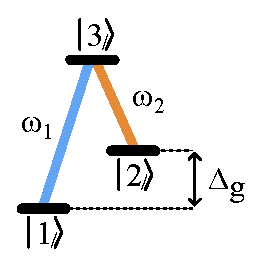
\includegraphics[width=0.2\linewidth]{lambda}}
        \hfill
    }
    \legend{Здесь $\Delta_g$---величина сверхтонкого расщепления основного состояния.}
    \caption[Этот текст попадает в названия рисунков в списке рисунков]{Уровни энергии и диаграмма}\label{fig:lambda}
\end{figure}
Возникающий эффект можно объяснить как результат взаимной интерференции темновых состояний атомов.
Темные состояния, иначе именуемые состояниями когерентного пленения населённостей --- КПН, в простейшем случае можно описать при помощи лямбда схемы уровней энергии изображенной на рисунке~\cref{fig:lambda}.
Например, когда система находится под действием бихроматического лазерного излучения в ней возможны следующие переходы $\ket{1}\leftrightarrow\ket{3}$ и $\ket{2}\leftrightarrow\ket{3}$, которые индуцируются электромагнитными волнами с частотами $\omega_1$ и $\omega_2$ соответственно.
Темным состоянием $\ket{NC}$ в этом случае будет являться состояние для которого выполняется $\bra{3}\hat{H}\ket{NC}=0$, где $\hat{H}$---гамильтониан системы под действием излучения.

При наличии двух встречных пучков каждый из них будет индуцировать своё КПН состояние $\ket{NC_1}$ и $\ket{NC_2}$.
Встречные волны, вследствие эффекта Доплера, будут взаимодействовать с противоположными по направлению движения скоростными группами атомов.
Чем ближе частоты лазерного излучения к частотам переходов в атоме, тем сильнее будут сближаться скоростные группы атомов на которые воздействуют пучки.
Когда частота лазерного излучения начинает совпадать с частотой атомных переходов, пучки воздействуют на общую скоростную группу.
Наводимые каждым пучком КПН состояния начинают интерферировать.
Результат возникающей интерференции зависит от поляризации пучков. 
Например, в случае линейно поляризованных пучков:
\begin{enumerate}[beginpenalty=10000]
    \item $\braket{NC_1|NC_2}=0$ ---
    \item $\braket{NC_1|NC_2}=1$ ---
\end{enumerate}
Такой тип резонанса может использоваться
Субдоплеровские резонансы основанные на эффекте КПН известны давно []. 
В данном случае возникновение эффекта связано не с резонансом КПН как таковым, а с интерференцией двух независимых КПН состояний.
Теоретическое обоснование наблюдаемого эффекта на основе численных расчетов было представлено в работе \autocite{hafiz2017}, однако отсутствовало аналитическое решение.
% Обзор, введение в тему, обозначение места данной работы в мировых исследованиях и~т.\:п., можно использовать ссылки на~другие работы~\autocite{Gosele1999161,Lermontov} (если их~нет, то~в~автореферате автоматически пропадёт раздел <<Список литературы>>).

\ifsynopsis
%Этот абзац появляется только в~автореферате.
%Для формирования блоков, которые будут обрабатываться только в~автореферате,
%заведена проверка условия \verb!\!\verb!ifsynopsis!.
%Значение условия задаётся в~основном файле документа (\verb!synopsis.tex! для
%автореферата).
\else
%Этот абзац появляется только в~диссертации.
%Через проверку условия \verb!\!\verb!ifsynopsis!, задаваемого в~основном файле
%документа (\verb!dissertation.tex! для диссертации), можно сделать новую
%команду, обеспечивающую появление цитаты в~диссертации, но~не~в~автореферате.
\fi

% {\progress}
% Этот раздел должен быть отдельным структурным элементом по
% ГОСТ, но он, как правило, включается в описание актуальности
% темы. Нужен он отдельным структурынм элемементом или нет ---
% смотрите другие диссертации вашего совета, скорее всего не нужен.

{\aim} данной работы является разработка аналитической модели описывающей переходы возникающие под действием бихроматического излучения.

Для~достижения поставленной цели необходимо было решить следующие {\tasks}:
\begin{enumerate}[beginpenalty=10000] % https://tex.stackexchange.com/a/476052/104425
  \item Получить аналитическое описание на основе лямбда схемы уровней энергии.
  \item Получить аналитическое решение для системы с учетом магнитных подуровней энергии.
  \item Исследовать, разработать, вычислить и~т.\:д. и~т.\:п.
\end{enumerate}

{\novelty}
\begin{enumerate}[beginpenalty=10000] % https://tex.stackexchange.com/a/476052/104425
  \item Впервые получено аналитическое решение описывающее форму линии субдоплеровского резонанса возникающего в поле встречных бихроматических лазерных пучков. \ldots
  \item Впервые получена система уравнений описывающая поведение уровней энергии в атоме с учетом магнитных подуровней под действием встречных бихроматических лазерных пучков.\ldots
\end{enumerate}

{\influence} \ldots

{\methods} \ldots

{\defpositions}
\begin{enumerate}[beginpenalty=10000] % https://tex.stackexchange.com/a/476052/104425
  \item Первое положение
  \item Второе положение
  \item Третье положение
  \item Четвертое положение
\end{enumerate}

{\reliability} полученных результатов обеспечивается \ldots \ Результаты находятся в соответствии с результатами, полученными другими авторами.


{\probation}
Основные результаты работы докладывались~на:
перечисление основных конференций, симпозиумов и~т.\:п.

{\contribution} Автор принимал активное участие \ldots

\ifnumequal{\value{bibliosel}}{0}
{%%% Встроенная реализация с загрузкой файла через движок bibtex8. (При желании, внутри можно использовать обычные ссылки, наподобие `\cite{vakbib1,vakbib2}`).
    {\publications} Основные результаты по теме диссертации изложены
    в~XX~печатных изданиях,
    X из которых изданы в журналах, рекомендованных ВАК,
    X "--- в тезисах докладов.
}%
{%%% Реализация пакетом biblatex через движок biber
    \begin{refsection}[bl-author, bl-registered]
        % Это refsection=1.
        % Процитированные здесь работы:
        %  * подсчитываются, для автоматического составления фразы "Основные результаты ..."
        %  * попадают в авторскую библиографию, при usefootcite==0 и стиле `\insertbiblioauthor` или `\insertbiblioauthorgrouped`
        %  * нумеруются там в зависимости от порядка команд `\printbibliography` в этом разделе.
        %  * при использовании `\insertbiblioauthorgrouped`, порядок команд `\printbibliography` в нём должен быть тем же (см. biblio/biblatex.tex)
        %
        % Невидимый библиографический список для подсчёта количества публикаций:
        \printbibliography[heading=nobibheading, section=1, env=countauthorvak,          keyword=biblioauthorvak]%
        \printbibliography[heading=nobibheading, section=1, env=countauthorwos,          keyword=biblioauthorwos]%
        \printbibliography[heading=nobibheading, section=1, env=countauthorscopus,       keyword=biblioauthorscopus]%
        \printbibliography[heading=nobibheading, section=1, env=countauthorconf,         keyword=biblioauthorconf]%
        \printbibliography[heading=nobibheading, section=1, env=countauthorother,        keyword=biblioauthorother]%
        \printbibliography[heading=nobibheading, section=1, env=countregistered,         keyword=biblioregistered]%
        \printbibliography[heading=nobibheading, section=1, env=countauthorpatent,       keyword=biblioauthorpatent]%
        \printbibliography[heading=nobibheading, section=1, env=countauthorprogram,      keyword=biblioauthorprogram]%
        \printbibliography[heading=nobibheading, section=1, env=countauthor,             keyword=biblioauthor]%
        \printbibliography[heading=nobibheading, section=1, env=countauthorvakscopuswos, filter=vakscopuswos]%
        \printbibliography[heading=nobibheading, section=1, env=countauthorscopuswos,    filter=scopuswos]%
        %
        \nocite{*}%
        %
        {\publications} Основные результаты по теме диссертации изложены в~\arabic{citeauthor}~печатных изданиях,
        \arabic{citeauthorvak} из которых изданы в журналах, рекомендованных ВАК\sloppy%
        \ifnum \value{citeauthorscopuswos}>0%
            , \arabic{citeauthorscopuswos} "--- в~периодических научных журналах, индексируемых Web of~Science и Scopus\sloppy%
        \fi%
        \ifnum \value{citeauthorconf}>0%
            , \arabic{citeauthorconf} "--- в~тезисах докладов.
        \else%
            .
        \fi%
        \ifnum \value{citeregistered}=1%
            \ifnum \value{citeauthorpatent}=1%
                Зарегистрирован \arabic{citeauthorpatent} патент.
            \fi%
            \ifnum \value{citeauthorprogram}=1%
                Зарегистрирована \arabic{citeauthorprogram} программа для ЭВМ.
            \fi%
        \fi%
        \ifnum \value{citeregistered}>1%
            Зарегистрированы\ %
            \ifnum \value{citeauthorpatent}>0%
            \formbytotal{citeauthorpatent}{патент}{}{а}{}\sloppy%
            \ifnum \value{citeauthorprogram}=0 . \else \ и~\fi%
            \fi%
            \ifnum \value{citeauthorprogram}>0%
            \formbytotal{citeauthorprogram}{программ}{а}{ы}{} для ЭВМ.
            \fi%
        \fi%
        % К публикациям, в которых излагаются основные научные результаты диссертации на соискание учёной
        % степени, в рецензируемых изданиях приравниваются патенты на изобретения, патенты (свидетельства) на
        % полезную модель, патенты на промышленный образец, патенты на селекционные достижения, свидетельства
        % на программу для электронных вычислительных машин, базу данных, топологию интегральных микросхем,
        % зарегистрированные в установленном порядке.(в ред. Постановления Правительства РФ от 21.04.2016 N 335)
    \end{refsection}%
    \begin{refsection}[bl-author, bl-registered]
        % Это refsection=2.
        % Процитированные здесь работы:
        %  * попадают в авторскую библиографию, при usefootcite==0 и стиле `\insertbiblioauthorimportant`.
        %  * ни на что не влияют в противном случае
       % \nocite{vakbib2}%vak
       % \nocite{patbib1}%patent
       % \nocite{progbib1}%program
       % \nocite{bib1}%other
       % \nocite{confbib1}%conf
    \end{refsection}%
        %
        % Всё, что вне этих двух refsection, это refsection=0,
        %  * для диссертации - это нормальные ссылки, попадающие в обычную библиографию
        %  * для автореферата:
        %     * при usefootcite==0, ссылка корректно сработает только для источника из `external.bib`. Для своих работ --- напечатает "[0]" (и даже Warning не вылезет).
        %     * при usefootcite==1, ссылка сработает нормально. В авторской библиографии будут только процитированные в refsection=0 работы.
}

% Счётчик \texttt{citeexternal} используется для подсчёта процитированных публикаций;
% \texttt{citeregistered} "--- для подсчёта суммарного количества патентов и программ для ЭВМ.

%Для добавления в список публикаций автора работ, которые не были процитированы в
%автореферате, требуется их~перечислить с использованием команды \verb!\nocite! в
%\verb!Synopsis/content.tex!.
